
\begin{frame}{(screaming)PYHA PAPER}
    \centering
    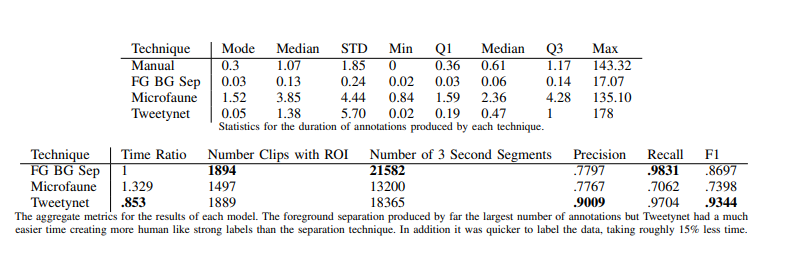
\includegraphics[height=1\textheight,width=1\textwidth,keepaspectratio]{model_performance_01_23.png}
\end{frame}

\begin{frame}{ICLR PAPER}
    \centering
    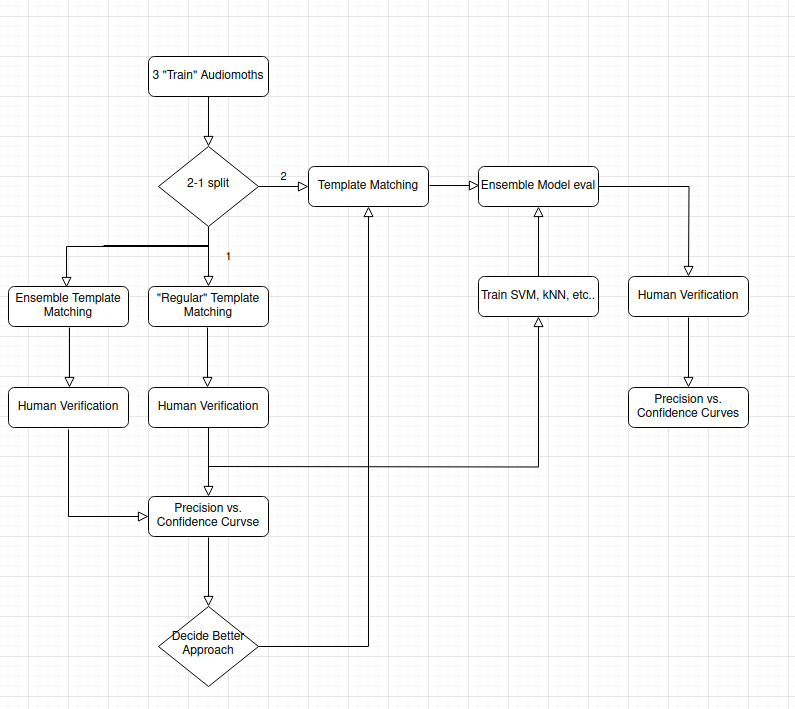
\includegraphics[height=0.7\textheight,width=0.7\textwidth,keepaspectratio]{ICLR_WORKFLOW.png}
\end{frame}

\begin{frame}{UCSC Collaboration - Template Matching}
    \begin{itemize}
        \item ( ) For labeling
        \item (X) For training
    \end{itemize}
\end{frame}

\begin{frame}{SoundSim}
    \centering
    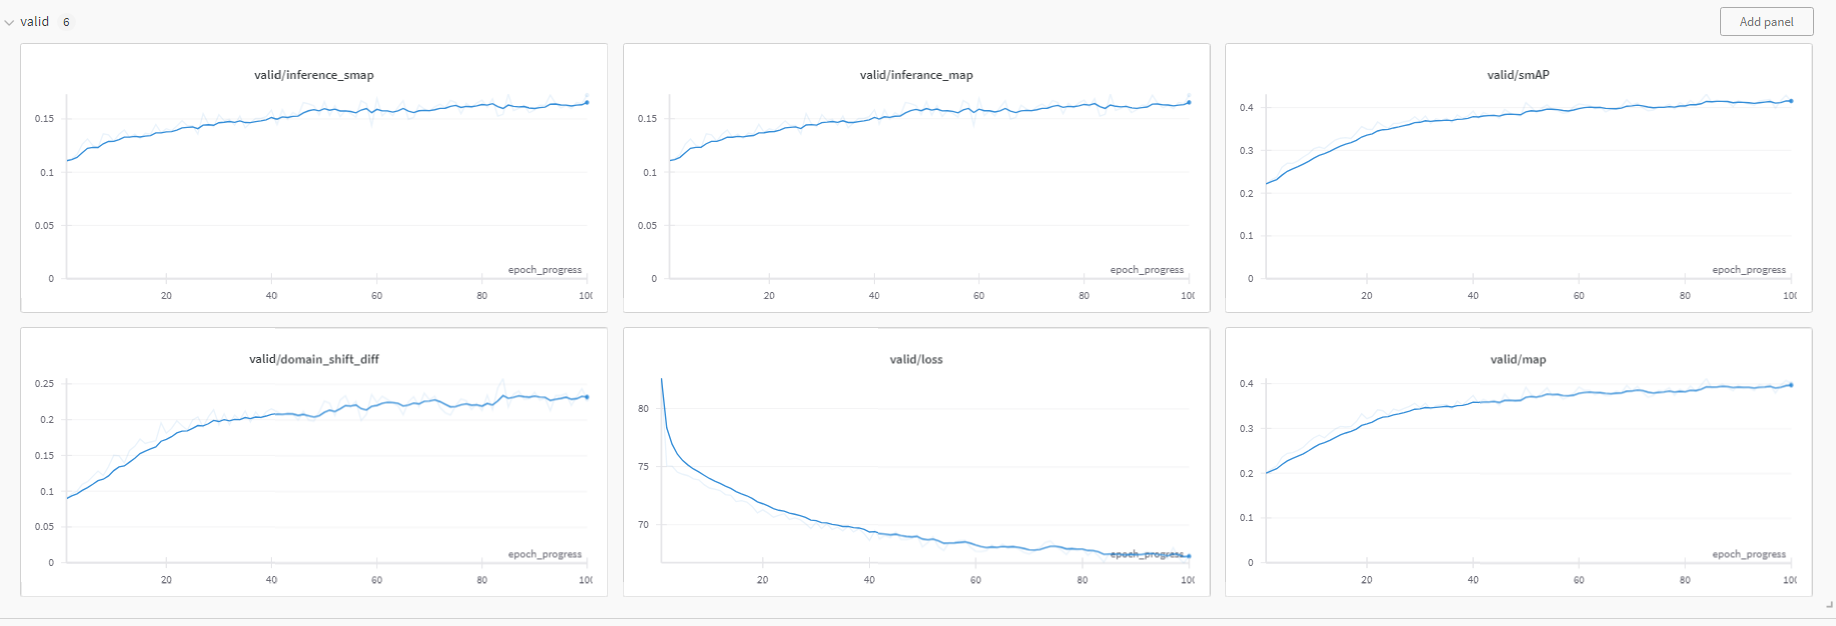
\includegraphics[height=1\textheight,width=1\textwidth,keepaspectratio]{sound_sim_baseline.png}
\end{frame}

\begin{frame}{IR Sim}
    \begin{itemize}
        \item IR integrated
        \item Testing before instances
    \end{itemize}
\end{frame}

\begin{frame}{Quarter Plans For San Diego Zoo}
    \begin{itemize}
        \item BIRB benchmark 
        \item Inference FG-BG separation
    \end{itemize}
\end{frame}

\begin{frame}{Dylan Thesis}
    \centering
    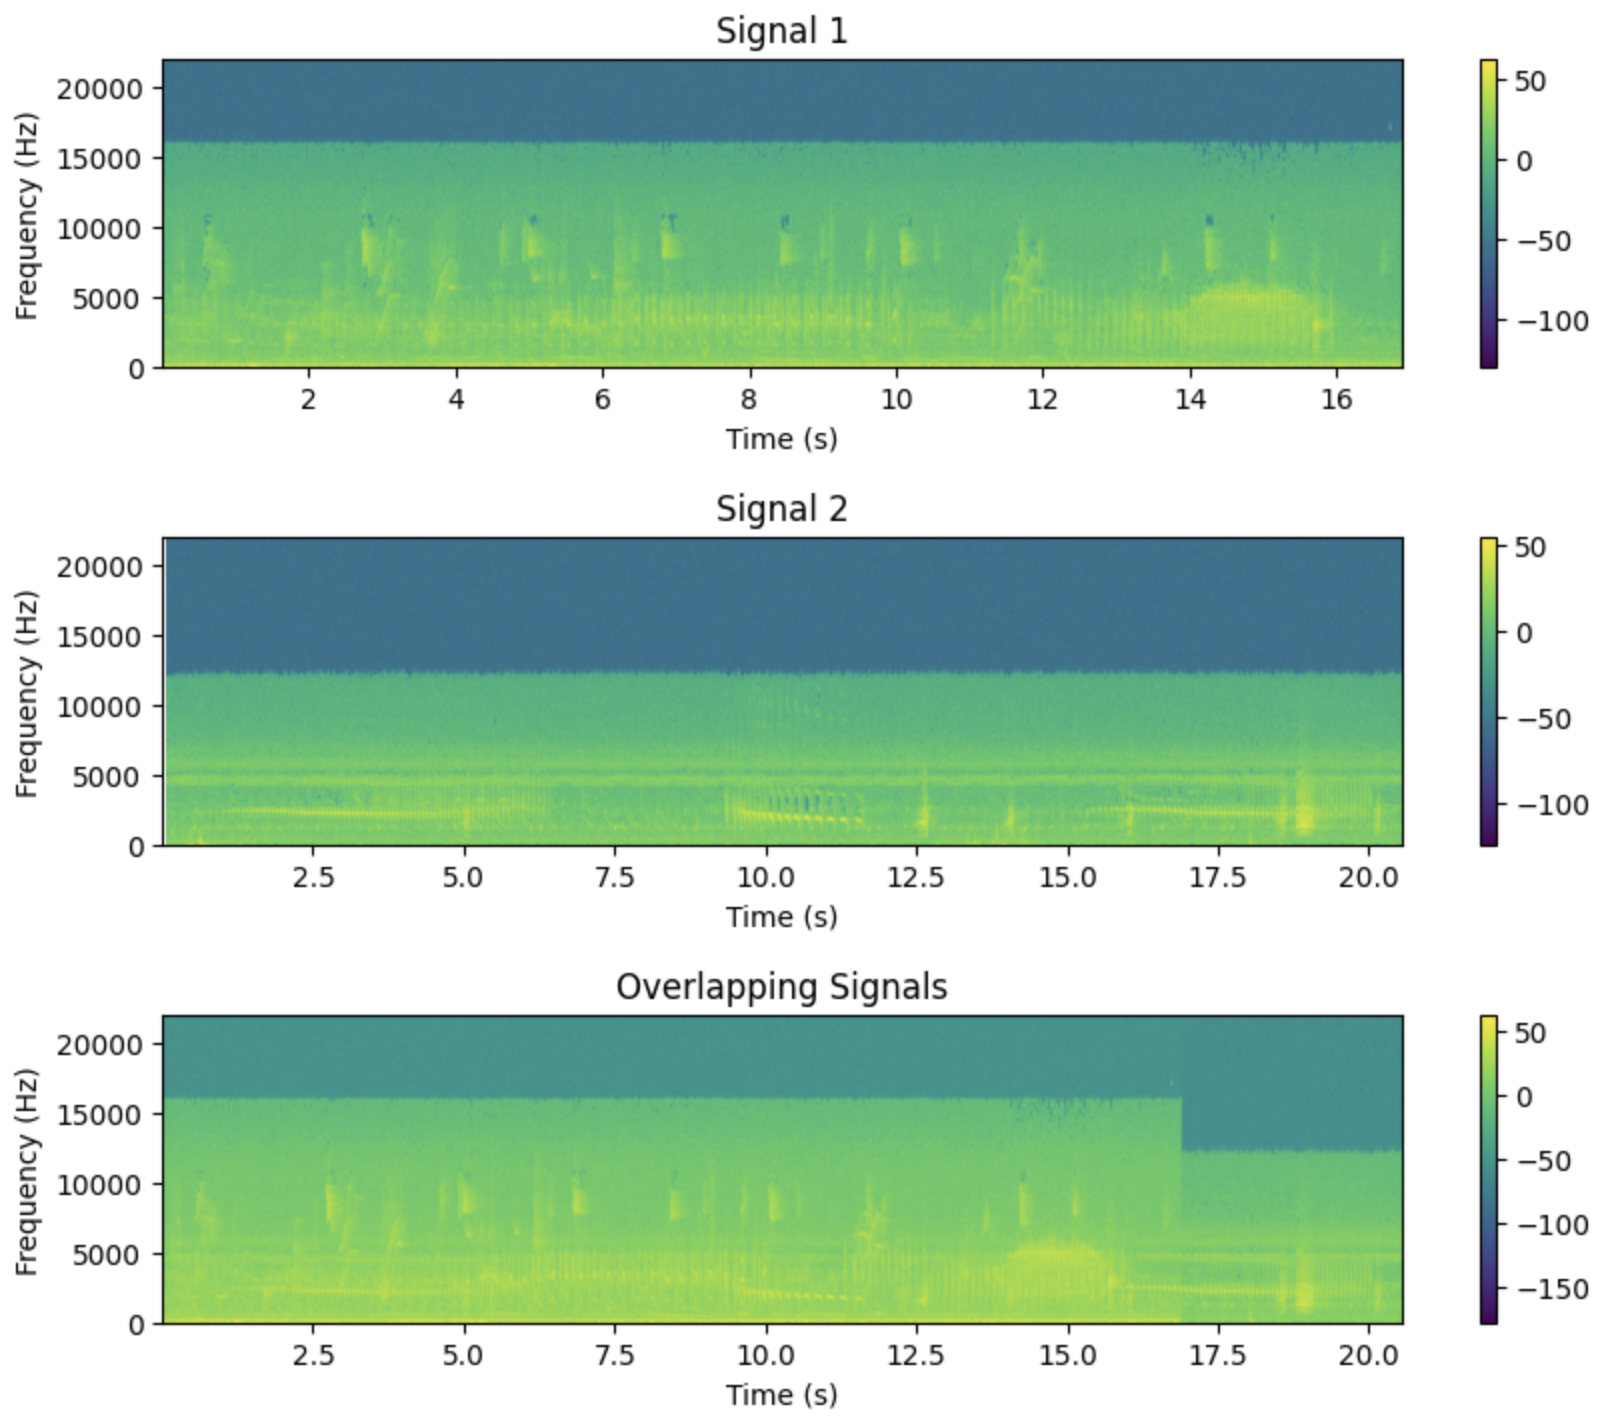
\includegraphics[height=0.7\textheight,width=0.7\textwidth,keepaspectratio]{dylan-aid-1-24.png}
\end{frame}





% Slides for 2024-01-24
% To create a slide, use the following:
% \begin{frame}{TITLE}
%     BODY
% \end{frame}

% To create a slide with a bullet list, use the following:
% \begin{frame}{TITLE}
%     \begin{itemize}
%         \item ITEM 1
%         \item ITEM 2
%     \end{itemize}    
% \end{frame}

% To create a slide with numbered list, use the following:
% \begin{frame}{TITLE}
%     \begin{enumerate}
%         \item ITEM 1
%         \item ITEM 2
%     \end{enumerate}
% \end{frame}

% To create a slide with a graphic:
% 1. Add the graphic to this folder (named picture.png)
% 2. Use the following:
% \begin{frame}{TITLE}
%     \centering
%     \includegraphics[height=0.7\textheight,width=0.7\textwidth,keepaspectratio]{picture.png}
% \end{frame}

% To create a slide with two columns, use the following:
% \begin{frame}{TITLE}
%     \begin{columns}
%         \begin{column}{0.5\textwidth}
%             COLUMN 1 BODY
%         \end{column}
%         \begin{column}{0.5\textwidth}
%             COLUMN 2 BODY
%         \end{column}
%     \end{columns}
% \end{frame}
